\documentclass[a4paper,11pt,fleqn]{article}%fleqn pour aligner les equations à gauche
\usepackage{../../Styles/Exercice}


\newcommand{\chnum}{Chapitre 1}
\newcommand{\chtitle}{Identification d'espèces chimiques}
\newcommand{\dtype}{Exercices}

\begin{document}
\maketitle

\begin{multicols}{2}
\section{Analyser des produits ménagers}
Il existe de très nombreux produits ménagers. Le vinaigre ménager, utilisé pour détartrer les robinetteries et les carrelages, contient de l'eau (\ce{H2O}) et \SI{14}{\percent} d'acide acétique (\ce{C2H4O2}). L'alcool à brûler, utilisé pour nettoyer les vitres, est constitué d'éthanol (\ce{C2H6O}), de méthanol (\ce{CH4O}) et d'eau (\ce{H2O}). L'ammoniaque, utilisée pour raviver les couleurs des tapis, est une solution qui contient de l'ammoniac (\ce{NH3}) dissous dans l'eau (\ce{H2O}). L'eau déminéralisée, utilisée pour éviter les dépôts de calcaire dans les fers à repasser, ne contient plus de minéraux (ions).
\begin{enumerate}
	\item Lister les espèces chimiques présentes dans ces produits ménagers.
	\item Ces produits ménagers sont-ils des corps purs ou des mélanges ?
\end{enumerate}

\section{Connaître la composition de l'air}
L'air est un mélange de gaz.
\begin{enumerate}
	\item Quels sont les deux gaz majoritaires présents dans l'air ?
	\item Quelle est al composition, exprimée en pourcentage, de l'air ?
	\item Calculer la masse, exprimée en gramme, d'un litre d'air.
\end{enumerate}

\textbf{Donnée :}\\
\textbf{Masse volumique de l'air :} $\rho_{air} =$ \SI{1,225}{\kilo\gram\per\meter\cubed} à \SI{15}{\celsius}.

\section{Représenter le contenu d'une éprouvette}
On introduit dans une éprouvette graduée \SI{20}{mL} d'eau et \SI{30}{mL} de cyclohexane. Ces deux liquides sont incolores et non miscibles entre eux.
\begin{itemize}
	\item Dessiner le contenu de l'éprouvette graduée.
\end{itemize}

\textbf{Données :}\\
\textbf{Densité de l'eau :} $d_{eau} =$ \SI{1,00}\\
\textbf{Densité du cyclohexane :} $d_{cyclohexane} =$ \SI{0,779}\\

\section{Identifier un liquide}
On place un tube à essai contenant un liquide $X$ dans un cristallisoir contenant un mélange réfrigérant (eau, glace et sel) et on mesure la température du liquide à intervalle de temps régulier.\\
La courbe donnant l'évolution de la température du liquide $X$ en fonction du temps est donnée ci-dessous.
\begin{enumerate}
	\item Pourquoi peut-on affirmer que ce corps est pur ?
	\item Déterminer la température de fusion du corps.
	\item En utilisant les données, en déduire le nom de ce corps pur.
\end{enumerate}
\begin{figure}[H]
    \centering
    \adjustbox{valign=b}{\subfloat[\textbf{Évolution de la température de $X$ au cours du temps}]{
    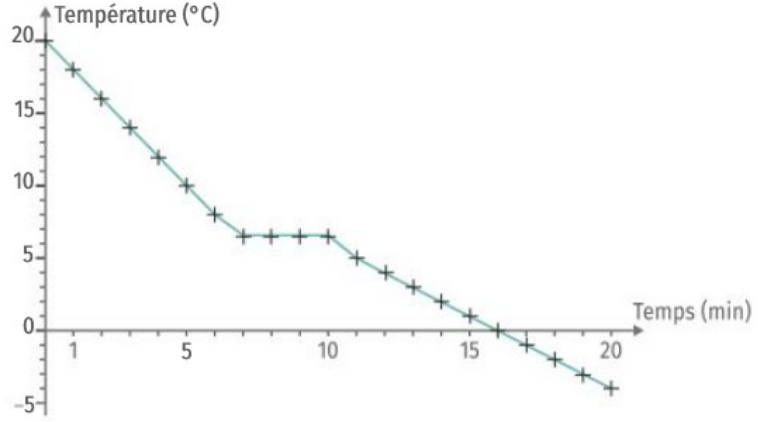
\includegraphics[scale=.35]{Ressources/2GT_C1_Ex_Fig1.png}}}
\end{figure}

\textbf{Données :}\\
\begin{tabular}{m{5cm}m{5cm}}
$\theta_{f,\text{eau}}$ = \SI{0}{\celsius} & $\theta_{f,\text{pental-3-ol}}$ = \SI{-8}{\celsius}\\
$\theta_{f,\text{éthanol}}$ = \SI{-114}{\celsius} & $\theta_{f,\text{benzène}}$ = \SI{5.5}{\celsius}\\
$\theta_{f,\text{cyclohexane}}$ = \SI{6.5}{\celsius} & $\theta_{f,\text{méthanamide}}$ = \SI{2.5}{\celsius}\\
$\theta_{f,\text{éther}}$ = \SI{-116}{\celsius}&\\
\end{tabular}

\section{Solution inconnue}
Rami a préparé une solution aqueuse et vous mer au défi de retrouver les ions présents dans cette solution.\\
Une série de tests a été réalisée et les résultats obtenus sont regroupés dans le tableau ci-dessous :\\
\begin{tabular}{|>{\centering}m{4.2cm}|>{\centering\arraybackslash}m{4.2cm}|}
\hline
\textbf{Réactif} & \textbf{Résultat du test}\\ \hline
Nitrate d'argent & Positif\\ \hline
Soude & Négatif\\ \hline
Chlorure de baryum & Négatif\\ \hline
Oxalate d'ammonium & Positif\\ \hline
\end{tabular}
\begin{enumerate}
	\item Faire un schéma type de l'expérience à réaliser pour faire ces tests.
	\item Déterminer la nature des ions présents dans la solution réalisée par Rami.
	\item La solution est-elle un corps pur ou un mélange ?
\end{enumerate}

\textbf{Tests d'ions en solution aqueuse :}\\
\begin{tabular}{|>{\centering}m{2.2cm}|>{\centering}m{2.8cm}|>{\centering\arraybackslash}m{3.2cm}|}
\hline
\textbf{Ion} & \textbf{Réactif utilisé} & \textbf{Observation}\\ \hline
Chlorure \ce{Cl-} &Nitrate d'argent & Précipité blanc qui noircit à la lumière\\ \hline
Cuivre II \ce{Cu^{2+}} & Soude & Précipité bleu\\ \hline
Fer II \ce{Fe^{2+}} & Soude & Précipité vert\\ \hline
Fer III \ce{Fe^{3+}} & Soude & Précipité orange\\ \hline
Calcium \ce{Ca^{2+}} & Oxalate d'ammonium & Précipité blanc\\ \hline
Sulfate \ce{SO4^{2-}} & Chlorure de baryum & Précipité blanc\\ \hline
Sodium \ce{Na+} & Test à la flamme & Flamme jaune\\ \hline
Potassium \ce{K+} & Test à la flamme & Flamme violette\\ \hline
\end{tabular}

\section{Le trimix}
Le trimix est un mélange de gaz utilisé pour al plongée. À partir des masse de chaque gaz contenu dans la bouteille, calculer le pourcentage en volume de chaque gaz dans le trimix.\\
\textbf{Données :}\\
\begin{tabular}{m{5cm}|m{3.5cm}}
\textbf{Pour une bouteille de \SI{12}{kg}} & \textbf{Masse volumique du gaz à pression atmosphérique :} \\
masse de dioxygène : \SI{3.3}{kg} & $\rho$(\ce{O2}) = \SI{1.33}{\gram\per\liter}\\
masse d'hélium : \SI{600}{g} & $\rho$(\ce{N2}) = \SI{1.17}{\gram\per\liter}\\
masse de diazote : \SI{8.1}{kg} & $\rho$(\ce{He}) = \SI{0.17}{\gram\per\liter}\\
\end{tabular}

\end{multicols}

\end{document}